\section{マルコフ連鎖モンテカルロ法 (MCMC)}
前節では解析的に事後分布の計算をした.事後分布を近似的に推論する方法の1つに\textbf{マルコフ連鎖モンテカルロ法 (Markov chain Monte Carlo methods; MCMC)} がある.他の近似推論の手法としてはLaplace近似や変分推論 (variational inference) などがある.MCMCは他の手法に比して,事後分布の推論だけでなく,確率分布を神経活動で表現する方法を提供するという利点がある.

\footnote{
変分推論は入れた方がいいと思うが,紙幅の都合上いれられるか微妙である.
}

データを$X$とし,パラメータを$\theta$とする.


\begin{equation}
p(\theta\mid X)=\frac{p(X\mid \theta)p(\theta)}{\int p(X\mid \theta)p(\theta)d\theta}
\end{equation}


分母の積分計算$\int p(X\mid \theta)p(\theta)d\theta$が求まればよい.

\subsubsection{モンテカルロ法}

\subsubsection{マルコフ連鎖}
\subsection{Metropolis-Hastings法}
\lstinputlisting[language=julia]{./text/bayesian-brain/mcmc/002.jl}
\lstinputlisting[language=julia]{./text/bayesian-brain/mcmc/003.jl}
\lstinputlisting[language=julia]{./text/bayesian-brain/mcmc/004.jl}
\begin{figure}[ht]
	\centering
	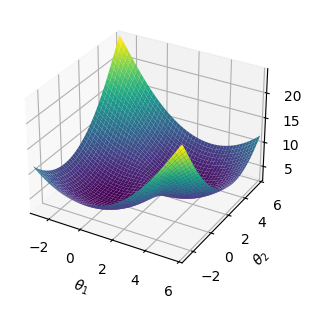
\includegraphics[scale=0.8, max width=\linewidth]{./fig/bayesian-brain/mcmc/cell004.png}
	\caption{cell004.png}
	\label{cell004.png}
\end{figure}
\lstinputlisting[language=julia]{./text/bayesian-brain/mcmc/005.jl}
\lstinputlisting[language=julia]{./text/bayesian-brain/mcmc/006.jl}
\lstinputlisting[language=julia]{./text/bayesian-brain/mcmc/007.jl}
\lstinputlisting[language=julia]{./text/bayesian-brain/mcmc/008.jl}
\lstinputlisting[language=julia]{./text/bayesian-brain/mcmc/009.jl}
\begin{figure}[ht]
	\centering
	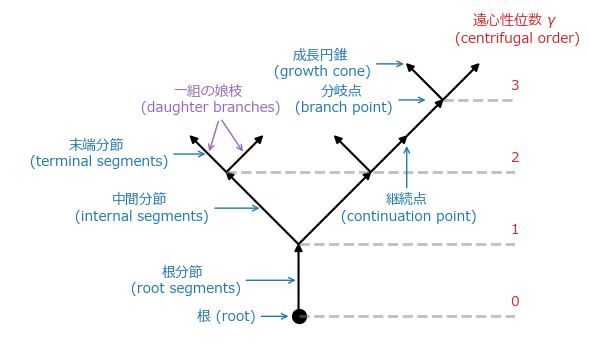
\includegraphics[scale=0.8, max width=\linewidth]{./fig/neuron-model/neurite-growth-model/cell009.png}
	\caption{cell009.png}
	\label{cell009.png}
\end{figure}
\subsection{ランジュバン・モンテカルロ法 (LMC)}
拡散過程


\begin{equation}
{\frac{d\theta}{dt}}=\nabla \log p (\theta)+{\sqrt 2}{d{W}}
\end{equation}


Euler–Maruyama法により,
\lstinputlisting[language=julia]{./text/bayesian-brain/mcmc/011.jl}
\lstinputlisting[language=julia]{./text/bayesian-brain/mcmc/012.jl}
\lstinputlisting[language=julia]{./text/bayesian-brain/mcmc/013.jl}
\lstinputlisting[language=julia]{./text/bayesian-brain/mcmc/014.jl}
\begin{figure}[ht]
	\centering
	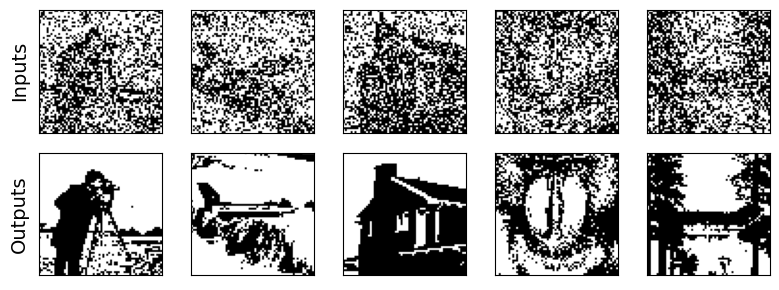
\includegraphics[scale=0.8, max width=\linewidth]{./fig/energy-based-model/hopfield-model/cell014.png}
	\caption{cell014.png}
	\label{cell014.png}
\end{figure}
\subsection{ハミルトニアン・モンテカルロ法 (HMC法)}
ハミルトニアン・モンテカルロ法(Hamiltonian Monte Calro)あるいはハイブリッド・モンテカルロ法(Hybrid Monte Calro)という

一般化座標を$\mathbf{q}$, 一般化運動量を$\mathbf{p}$とする.ポテンシャルエネルギーを$U(\mathbf{q})$としたとき,古典力学 (解析力学) において保存力のみが作用する場合の\textbf{ハミルトニアン (Hamiltonian)} $\mathcal{H}(\mathbf{q}, \mathbf{p})$は


\begin{equation}
\mathcal{H}(\mathbf{q}, \mathbf{p}):=U(\mathbf{q})+\frac{1}{2}\|\mathbf{p}\|^2
\end{equation}


となる.このとき,次の2つの方程式が成り立つ.


\begin{equation}
\frac{d\mathbf{q}}{dt}=\frac{\partial \mathcal{H}}{\partial \mathbf{p}}=\mathbf{p},\quad\frac{d\mathbf{p}}{dt}=-\frac{\partial \mathcal{H}}{\partial \mathbf{q}}=-\frac{\partial U}{\partial \mathbf{q}}
\end{equation}


これを\textbf{ハミルトンの運動方程式(hamilton's equations of motion)} あるいは\textbf{正準方程式 (canonical equations)} という.


この処理をMetropolis-Hastings法における採用・不採用アルゴリズムという.

リープフロッグ(leap frog)法により離散化する.
\lstinputlisting[language=julia]{./text/bayesian-brain/mcmc/016.jl}
\lstinputlisting[language=julia]{./text/bayesian-brain/mcmc/017.jl}
\lstinputlisting[language=julia]{./text/bayesian-brain/mcmc/018.jl}
\lstinputlisting[language=julia]{./text/bayesian-brain/mcmc/019.jl}
\lstinputlisting[language=julia]{./text/bayesian-brain/mcmc/020.jl}
\begin{figure}[ht]
	\centering
	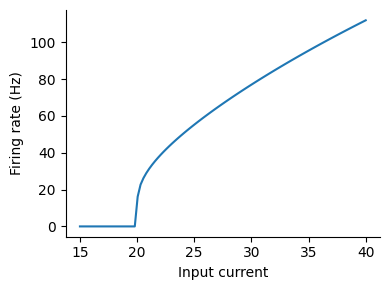
\includegraphics[scale=0.8, max width=\linewidth]{./fig/neuron-model/lif/cell020.png}
	\caption{cell020.png}
	\label{cell020.png}
\end{figure}
*ToDo: 自己相関確認する*
\subsection{線形回帰への適応}
\lstinputlisting[language=julia]{./text/bayesian-brain/mcmc/023.jl}
\lstinputlisting[language=julia]{./text/bayesian-brain/mcmc/024.jl}
\lstinputlisting[language=julia]{./text/bayesian-brain/mcmc/025.jl}
\lstinputlisting[language=julia]{./text/bayesian-brain/mcmc/026.jl}
\lstinputlisting[language=julia]{./text/bayesian-brain/mcmc/027.jl}
\lstinputlisting[language=julia]{./text/bayesian-brain/mcmc/028.jl}
\lstinputlisting[language=julia]{./text/bayesian-brain/mcmc/029.jl}
\lstinputlisting[language=julia]{./text/bayesian-brain/mcmc/030.jl}
\begin{figure}[ht]
	\centering
	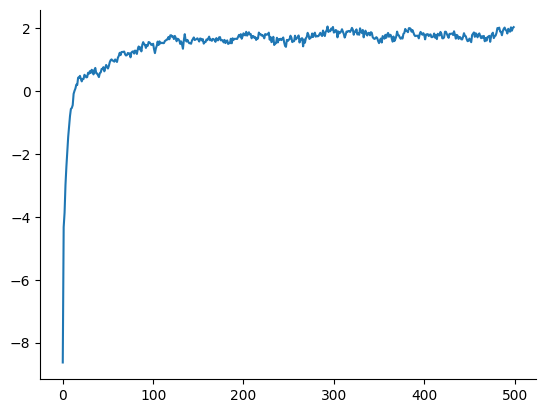
\includegraphics[scale=0.8, max width=\linewidth]{./fig/bayesian-brain/mcmc/cell030.png}
	\caption{cell030.png}
	\label{cell030.png}
\end{figure}
\lstinputlisting[language=julia]{./text/bayesian-brain/mcmc/031.jl}
\lstinputlisting[language=julia]{./text/bayesian-brain/mcmc/032.jl}
\begin{figure}[ht]
	\centering
	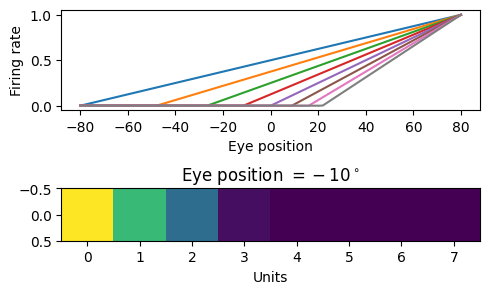
\includegraphics[scale=0.8, max width=\linewidth]{./fig/solve-credit-assignment-problem/backpropagation/cell032.png}
	\caption{cell032.png}
	\label{cell032.png}
\end{figure}
